\documentclass[11pt]{article}
\usepackage{graphicx} % Required for inserting images
\usepackage{tabularx}
\usepackage{algorithm}
\usepackage{changepage}
\usepackage{amsmath}
\usepackage{pgfplots}
\usepackage{algpseudocode}
\usepackage[a4paper,
            left=1in,
            top=1.5in,
            right=1in]{geometry}
\usepackage{listings}
\usepackage{color}

\definecolor{dkgreen}{rgb}{0,0.6,0}
\definecolor{gray}{rgb}{0.5,0.5,0.5}
\definecolor{mauve}{rgb}{0.58,0,0.82}

\lstset{frame=tb,
  language=Java,
  aboveskip=3mm,
  belowskip=3mm,
  showstringspaces=false,
  columns=flexible,
  basicstyle={\small\ttfamily},
  numbers=none,
  numberstyle=\tiny\color{gray},
  keywordstyle=\color{blue},
  commentstyle=\color{dkgreen},
  stringstyle=\color{mauve},
  breaklines=true,
  breakatwhitespace=true,
  tabsize=3
}

\title{Networked software for distributed systems\\Project 2}
\date{2022-2023}

\begin{document}

\begin{titlepage}
\begin{center}
		\begin{figure}[ht]
			\centering
\includegraphics[width=0.7\textwidth]{resources/Logo_Politecnico_Milano.png}
		\end{figure}
        
        \vspace{3.5cm}

        \LARGE
        \textit{Networked software for distributed systems}\\

        \vspace{0.5cm}
        \Large
        \textbf{Analysis of COVID-19 Data}
        
        \vspace{\fill}
  
		\large
		\begin{tabularx}{\linewidth}{@{}lXl@{}}
			\textit{Authors:}  & & \textit{Professors:} \\
			Stefano Carraro      & & Prof.\@ Luca Mottola\\
			Stefano Fossati  & & Prof. Alessandro Margara \\
			Andrea Restelli & & \\
		\end{tabularx}		
		\thispagestyle{empty}

        \vspace{1cm}

        2022-2023
           
\end{center}
\end{titlepage}

\tableofcontents
\cleardoublepage

%%%
\section{Introduction}
\subsection{Request}
\subsubsection{Description}
In a smart home, a control panel provides a user interface to coordinate the operation of several home appliances, such as HVAC systems, kitchen machines, and in-house entertainment, based on environmental conditions gathered through sensors. Users input to the control panel their preferences, e.g., the desired room temperature. Based on information returned by every appliance, the control panel offers information on the instantaneous energy consumption over the Internet. You are to implement the software layer for the smart home using the actor model. Every appliance may come and go depending on its operational times. The processes in charge of managing every appliance may also crash unpredictably. You need to demonstrate at least three example executions that include: 
\begin{enumerate}
\item the user inputting some preferences,  

\item sensors producing some (dummy) values, and  

\item appliances changing their behavior based on 1. and 2.  
\end{enumerate}
The three example executions must be able to operate in parallel in two or more rooms of the same smart home and tolerate process crashes.  
\subsubsection{Assumption and Guidelines}
\begin{enumerate}
    \item Although processes can crash, you can assume that channels are reliable. 

\item You are allowed to use any Akka facility, including the clustering/membership service. 

\item Sensors, appliances and the control panel may be emulated via software with dummy data. 
\end{enumerate}

\subsubsection{Technologies}
Akka

\subsection{Additional Assumption}
If the user interface for inserting commands into the application crashes it is manually restarted. 

%%%%

\cleardoublepage


\section{Design}
\subsection{Application Architecture}
The following figure shows the components of the application and their interconnections.
$\\$
Since Akka relies on the Actor Model, each element represented below correspond to an Actor in our application in order to exchange messages.

\begin{figure}[h]
\centering
    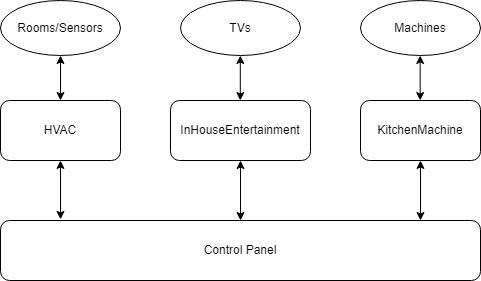
\includegraphics[width=0.6\linewidth]{resources/Design.png} 
    \caption{Application Architecture}
\end{figure}
From the Control Panel the user can perform the following operations:
\begin{itemize}
    \item Create a new Room, TV, Machine or remove an existing one
    \item Show Sensors, TVs or Machines connected 
    \item Set the desired temperature in a room
    \item Turn on/off TVs or Machines
    \item Request the total energy consumption
    \item Make a Sensor, TV or Machine crash
    \item Make HVAC, InHouseEntertainment or KitchenMachine crash
\end{itemize}
After the user select what to do a message will be sent to the respective HVACActor, InHouseEntertainmentActor, KitchenMachineActor that will handle the request. 
$\\$
From now on we will refer as ServerActor to HVACActor, InHouseEntertainmentActor or KitchenMachineActor. ClientActor will refer aswell to ClientActorHVAC, ClientActorIHE or ClientActorKM.

\subsection{Control Panel Structure}
The Command Interface serves as the user
interface for inserting commands into the application.
The structure of the Control Panel is the following:
\begin{figure}[H]
\centering
    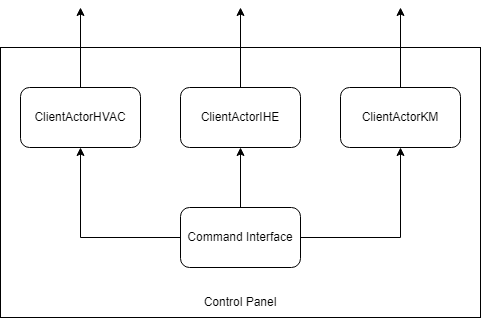
\includegraphics[width=0.6\linewidth]{resources/Panel.png} 
    \caption{Control Panel Structure}
    \label{fig:boat1}
\end{figure}
$\\$
The inserted command is then delivered to its respective ClientActor, which initiates the operation by communicating with the ServerActor.
$\\$
It would've worked aswell with a single client actor, but we've preferred to split them by areas of interest and threat them separately: this allows an easier scalability if a new feature with new devices needs to be added.

\subsection{Achieve Fault Tollerance}
It's necessary to define a supervisor and a strategy in order to handle process crashes. In this case the supervisor of the devices is the ServerActor itself: 
\begin{itemize}
    \item the HVACActor is the supervisor of all the sensors. 
    \item the InHouseEntertainmentActor is the supervisor of all the TVs. 
    \item the KitchenMachineActor is the supervisor of all the machines.
\end{itemize}
$\\$
Each ServerActor is then supervised by another supervisor. Resulting in the following hierarchy: 
$\\$
\begin{figure}[H]
\centering
    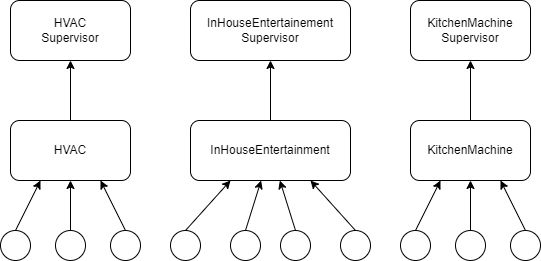
\includegraphics[width=0.8\linewidth]{resources/Hierarchy.png} 
    \caption{Supervisors Hierarchy}
\end{figure}
$\\$
The strategy adopted is the same by all of the three supervisors. When a device crashes it throws a CustomException and its supervisor apply the following strategy:
$\\$
\begin{lstlisting}[language=Java]
    private static SupervisorStrategy strategy =
            new OneForOneStrategy(
                    10,
                    Duration.ofMinutes(1),
                    DeciderBuilder.match(CustomException.class, e -> SupervisorStrategy.resume())
                            .build());

    @Override
    public SupervisorStrategy supervisorStrategy(){
        return strategy;
    }
\end{lstlisting}  
$\\$
The strategy is applied only on the crashing device and will try to resume it 10 times within a minute.

\section{Implementation}
\subsection{Starting Servers}
When a server is started it creates its own system, reading its corresponding configuration file. To achieve the hierarchy  described above it is necessary to create the supervisor first and then delegate it to create the ServerActor, this because of 
when an Actor create a new one. 
\subsection{Device Creation and Removal}
When a new device is inserted in the application it is necessary to instantiate it as a new Actor.
Let's assume we want to add a new television, and its ID is "TV1".
$\\$
In this case, a message (CreateDeviceMessage) is sent from the Control Panel to the InHouseEntertainmentActor. The ServerActor checks that the ID is unique and creates a new actor. The ActorRef, the reference to that actor, is saved so that the ServerActor knows where to send messages when required.
$\\$
When we want to remove a device, the corresponding ServerActor checks for the ID of the requested device, retrieves its ActorRef, and proceeds to stop the corresponding actor. This ensures that there won't be any issues if a device is removed while it is active. The ServerActor then unsave that ActorRef. 
$\\$

\subsection{HVAC and Sensors Implementation}
When a new room is added, the temperature is randomly set between 10.0°C and 25.0°C.
The HVACActor keeps track of all the room temperatures, while sensors only retrieve values.
$\\$
To emulate this process and generate realistic data, sensors need to remember their state, but that value is only used to produce data. This because to modify the temperature retrieved sensors have to work also as actuator (e.g., heat pump).
Once a desired temperature is requested for a specific room, the HVACActor saves the desired temperature value for that room, and the temperature increases or decreases until it matches the requested value.
$\\$
The following steps outline the process:

\begin{enumerate}
    \item The HVACActor instructs the sensor to increase or decrease the temperature.
    \item The sensor schedule a task that modifies the temperature every 3 seconds based on the previous request and send the calculated value to the HVACActor.
$\\$
    The temperature is increased or decreased by a \textit{dT} = 0.1°C.
    \item The HVACActor compare the current temperature value with the desired one. If they’re equal then it notices the sensor to stops, otherwise it lets the sensor continues.
\end{enumerate}    
If the desired temperature changes before its value is reached, the HVACActor notifies the sensor only if it is necessary to switch the operation applied (e.g., if the value was increasing, it will start decreasing).


\subsection{InHouseEntertainment and KitchenMachine implementation}
InHouseEntertainment and KitchenMachine operates under the same logic.
TVs and Machines can be turned on and off. 
When a new device is inserted it is set by default to off.
Once a device is turned on, as in HVAC, it schedule a task that send message to its corresponding ServerActor.
$\\$
When the device is turned off, the corresponding ServerActor instructs the device to change its state and cancels the task. When the device is inactive, it does not send any messages to the ServerActor.
This allows for proper functionality even in a scenario where the devices can be turned on using their physical buttons and not just from the control panel.

\subsection{Energy Consumption}
It is necessary to keep track of the energy consumption. We assume that each device of the same type consumes the same amount of energy in the same amount of time. 
$\\$
The following table shows the energy consumption values assigned to each device:
\begin{table}[H]
\centering
\begin{tabular}{|l|l|}
\hline
\textit{Device}  & \textit{dE}  \\ \hline
\textit{Sensor}  & \textit{10W} \\ \hline
\textit{TV}      & \textit{1W}  \\ \hline
\textit{Machine} & \textit{5W}  \\ \hline
\end{tabular}
\end{table}
$\\$
When each of the ServerActor receive a message from an operative device (the one sent during the task that we discussed before) it just increase the energy consumed by the respective \textit{dE} value.
For example, if a room is at 23.0°C and we desire a temperature of 24.0°C, it will send a total of 10 messages before the server stops the task, resulting in a total energy consumption of 100W.

\end{document}
